\section{Einleitung und Versuchsziel}
\label{sec:aufgabenstellung}
%In der Aufgabenstellung wird (in eigenen Worten und ganzen Sätzen) formuliert, was das Ziel des 
%Versuches ist.  
%[Beachten Sie die eigentliche Aufgabenstellung in den Versuchsanleitungen sowie die Hinweise zur Auswertung!] 

Für eine Arbeit des \textsc{Polymerservice Merseburg (PSM)} wird ein 2L-Reaktorsystem mit automatischer Dosierung über mehrere Stunden gefordert. Weiterhin sollen über Temperaturprofile Aufheiz- und Abkühlvorgänge gesteuert werden. Beide Anforderungen sind für zwei verschiedene Polymerisationen zu erfüllen, jedoch wird sich in dieser Arbeit auf den ersten der beiden Prozesse konzentriert. 

Ziel des Projektes im Rahmen des Moduls Thermischer Verfahrenstechnik II ist es, dass in Form einer studentischen Arbeit ein Prototyp für ein mögliches Reaktorsystem aufgebaut und vorgestellt wird. Die benötigten Spezifikationen an das geforderte System wurden hierfür abstrahiert und vereinfacht (vgl. Abb. \ref{fig:prozess 1} und Tab. \ref{tab:verinfachteAnforderungen}). Dabei wird aufgezeigt welche Möglichkeiten in der Umsetzung mit bereits vorhandenen Mitteln an der \textsc{Hochschule Merseburg} bestehen.

\begin{table}[h!]
	\renewcommand*{\arraystretch}{1.2}
	\centering
	\rowcolors{2}{gray!25}{white}
	\caption{zusammengefasste Anforderungen Prozess 1 und 2}
	\label{tab:Anforderungen1_2}
	\resizebox{\textwidth}{!}{
		\begin{tabulary}{1.15\textwidth}{L|L}
			\hline
			\textbf{Anforderung} & \textbf{Beschreibung}\\
			\hline
			2L-Reaktor &  Es wird ein 2L-Reaktor für die Reaktion benötigt. \\
			Temperaturprofile & Die Temperaturen des Prozesses sind über Temperaturprofile einzustellen.\\
			Feed 1 zu dosieren & Feed 1 ist mit \SI{135}{\milli \liter \per \hour} über \SI{3}{\hour} zuzudosieren.\\
			Feed 4 zu dosieren & Feed 4 ist mit \SI{20}{\milli \liter \per \hour} über \SI{1}{\hour} zuzudosieren.\\
			Feed 3 \& Feed 4 & Feed 3 und 4 werden nicht ausgeführt.\\
			Edukte & Wasser wird als Ersatz für die realen Edukte genutzt.\\
			Ankerrührer & Für die Durchmischung ist ein Ankerrührer zu verwenden.\\
			Stickstoffatmosphäre & Es wird keine Schutzatmosphäre ausgeführt.\\
			Wasserdampfdestillation & Es wird keine Wasserdampfdestillation ausgeführt.\\
			Kühler & Es wird keine Kühlung ausgeführt und kein Kondensat aufgefangen.\\
			\hline			
	\end{tabulary}}
\end{table}%
\FloatBarrier
\anmerkung{Tabelle Überarbeiten !!}

\begin{figure}[h!]
	\centering
	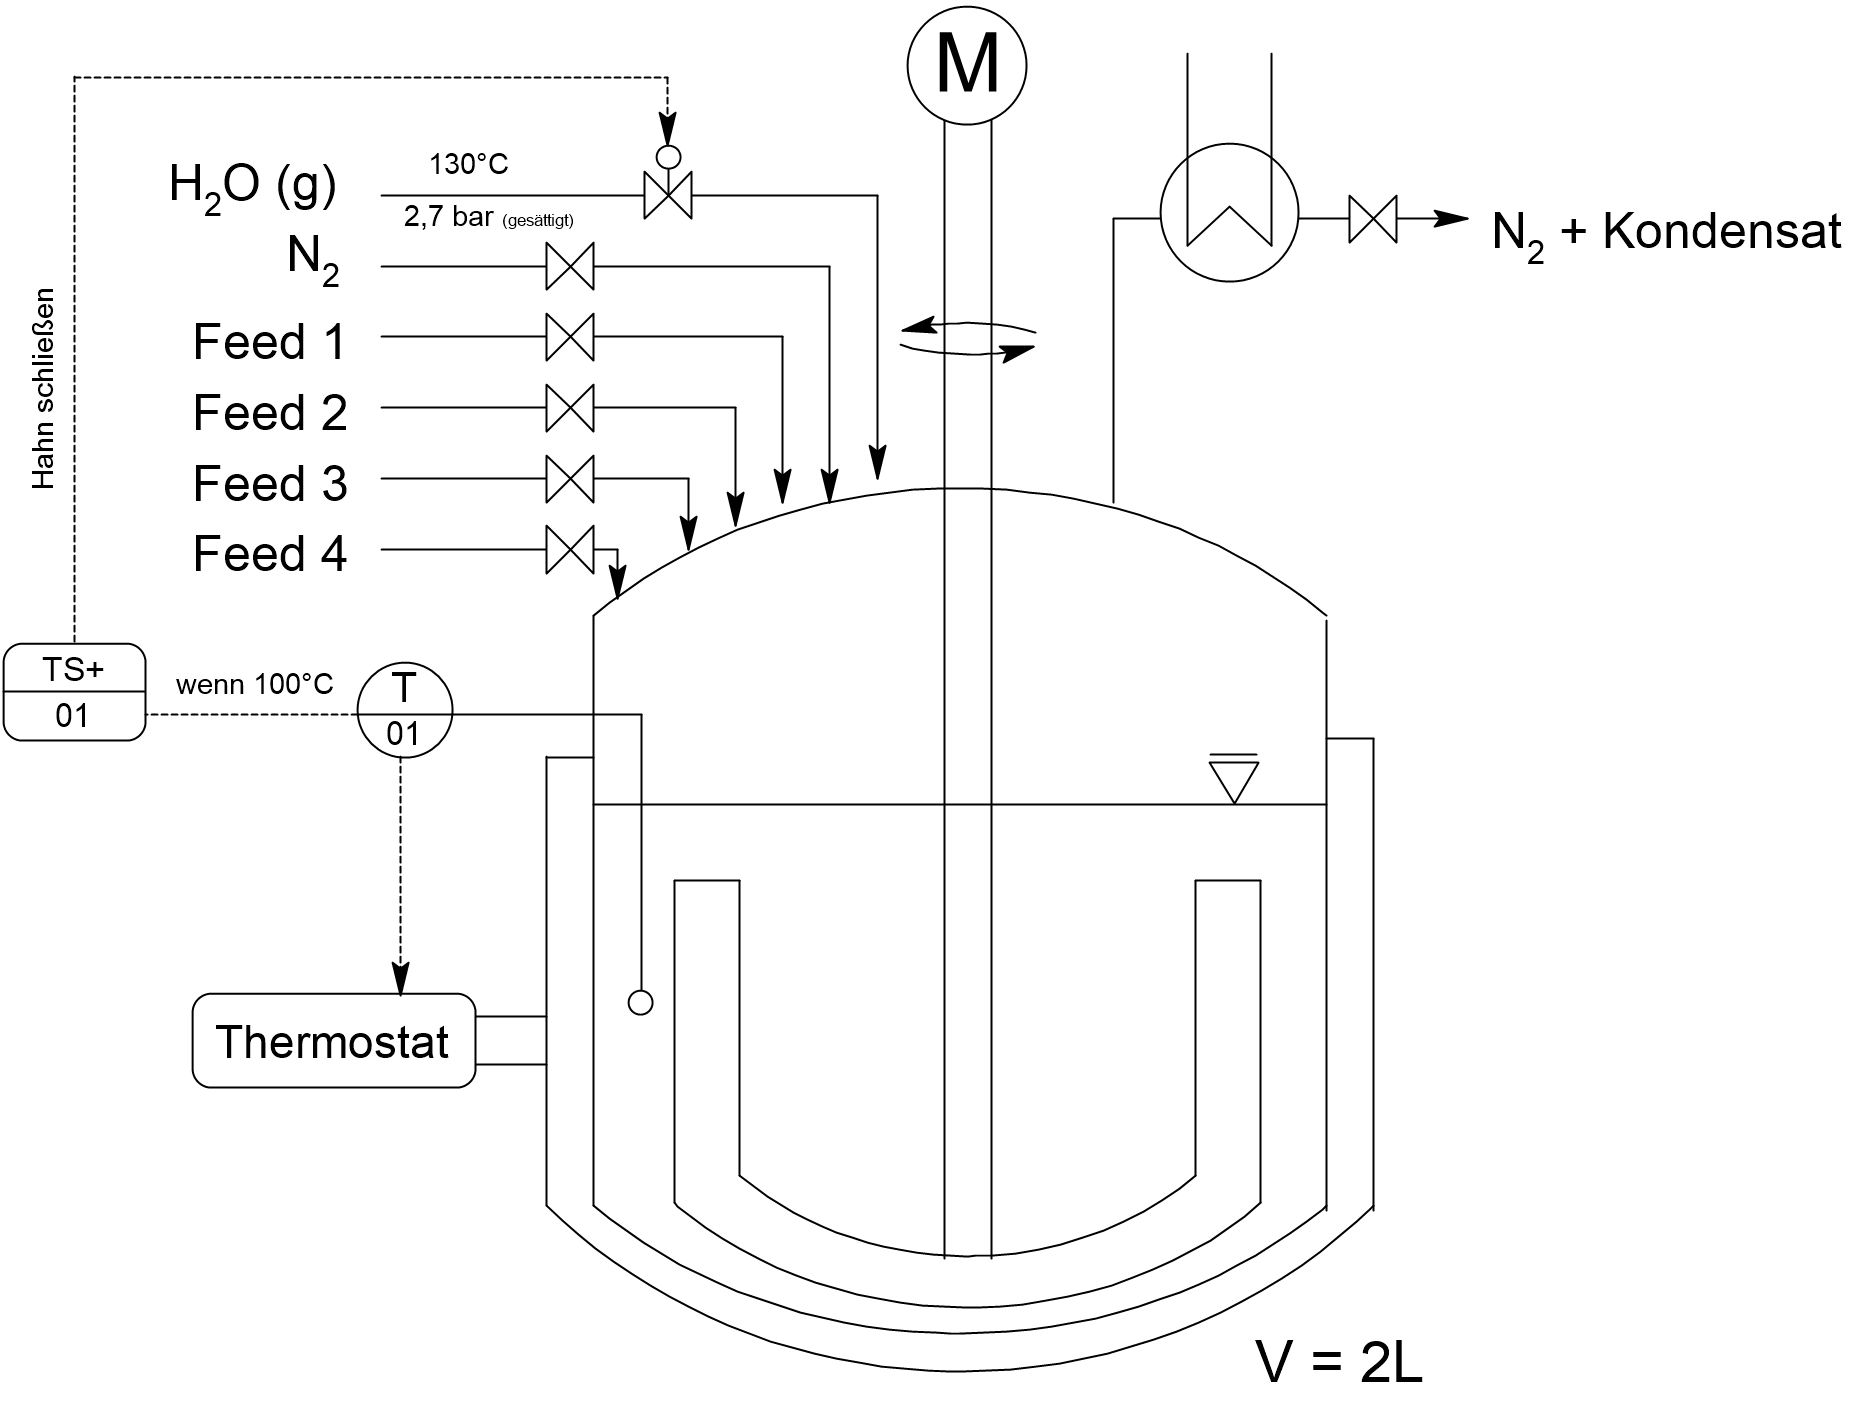
\includegraphics[width=0.75\textwidth]{img/Skizze_Prozess_1.png}
	\caption{Skizze der realen Anforderungen an den Prozess 1}
	\label{fig:prozess 1}
\end{figure}
\FloatBarrier
%Ende

\begin{table}[h!]
	\renewcommand*{\arraystretch}{1.2}
	\centering
	\rowcolors{2}{gray!25}{white}
	\caption{vereinfachte Anforderungen des Prozesses 1}
	\label{tab:verinfachteAnforderungen}
	\resizebox{\textwidth}{!}{
		\begin{tabulary}{1.15\textwidth}{L|L}
			\hline
			\textbf{Anforderung} & \textbf{Beschreibung}\\
			\hline
			2L-Reaktor &  Es wird ein 2L-Reaktor für die Reaktion benötigt. \\
			Temperaturprofile & Die Temperaturen des Prozesses sind über Temperaturprofile einzustellen.\\
			Feed 1 zu dosieren & Feed 1 ist mit \SI{135}{\milli \liter \per \hour} über \SI{3}{\hour} zuzudosieren.\\
			Feed 4 zu dosieren & Feed 4 ist mit \SI{20}{\milli \liter \per \hour} über \SI{1}{\hour} zuzudosieren.\\
			Feed 3 \& Feed 4 & Feed 3 und 4 werden nicht ausgeführt.\\
			Edukte & Wasser wird als Ersatz für die realen Edukte genutzt.\\
			Ankerrührer & Für die Durchmischung ist ein Ankerrührer zu verwenden.\\
			Stickstoffatmosphäre & Es wird keine Schutzatmosphäre ausgeführt.\\
			Wasserdampfdestillation & Es wird keine Wasserdampfdestillation ausgeführt.\\
			Kühler & Es wird keine Kühlung ausgeführt und kein Kondensat aufgefangen.\\
			\hline			
	\end{tabulary}}
\end{table}%
\FloatBarrier